% header
\documentclass[10pt,a4paper]{article}

\usepackage[utf8]{inputenc}
\usepackage{hyperref}
\usepackage{amssymb}
\usepackage{amsmath}
\usepackage{listings}
\usepackage{graphicx}

% the document
\begin{document}

\title{Worksheet $4$\\
\small{Practical Lab Numerical Computing}}
\author{Andrii Lischishin \and Lars Schleithoff \and Hendrik Kleikamp}
\date{\today}
\maketitle

\section*{Task 1}

\begin{center}
	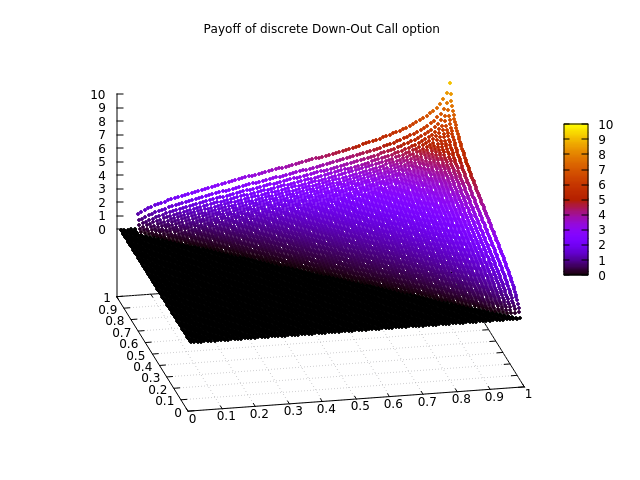
\includegraphics[scale=0.7]{images/payoff_down_out_call.png}
\end{center}

\section*{Task 2}


\begin{center}
	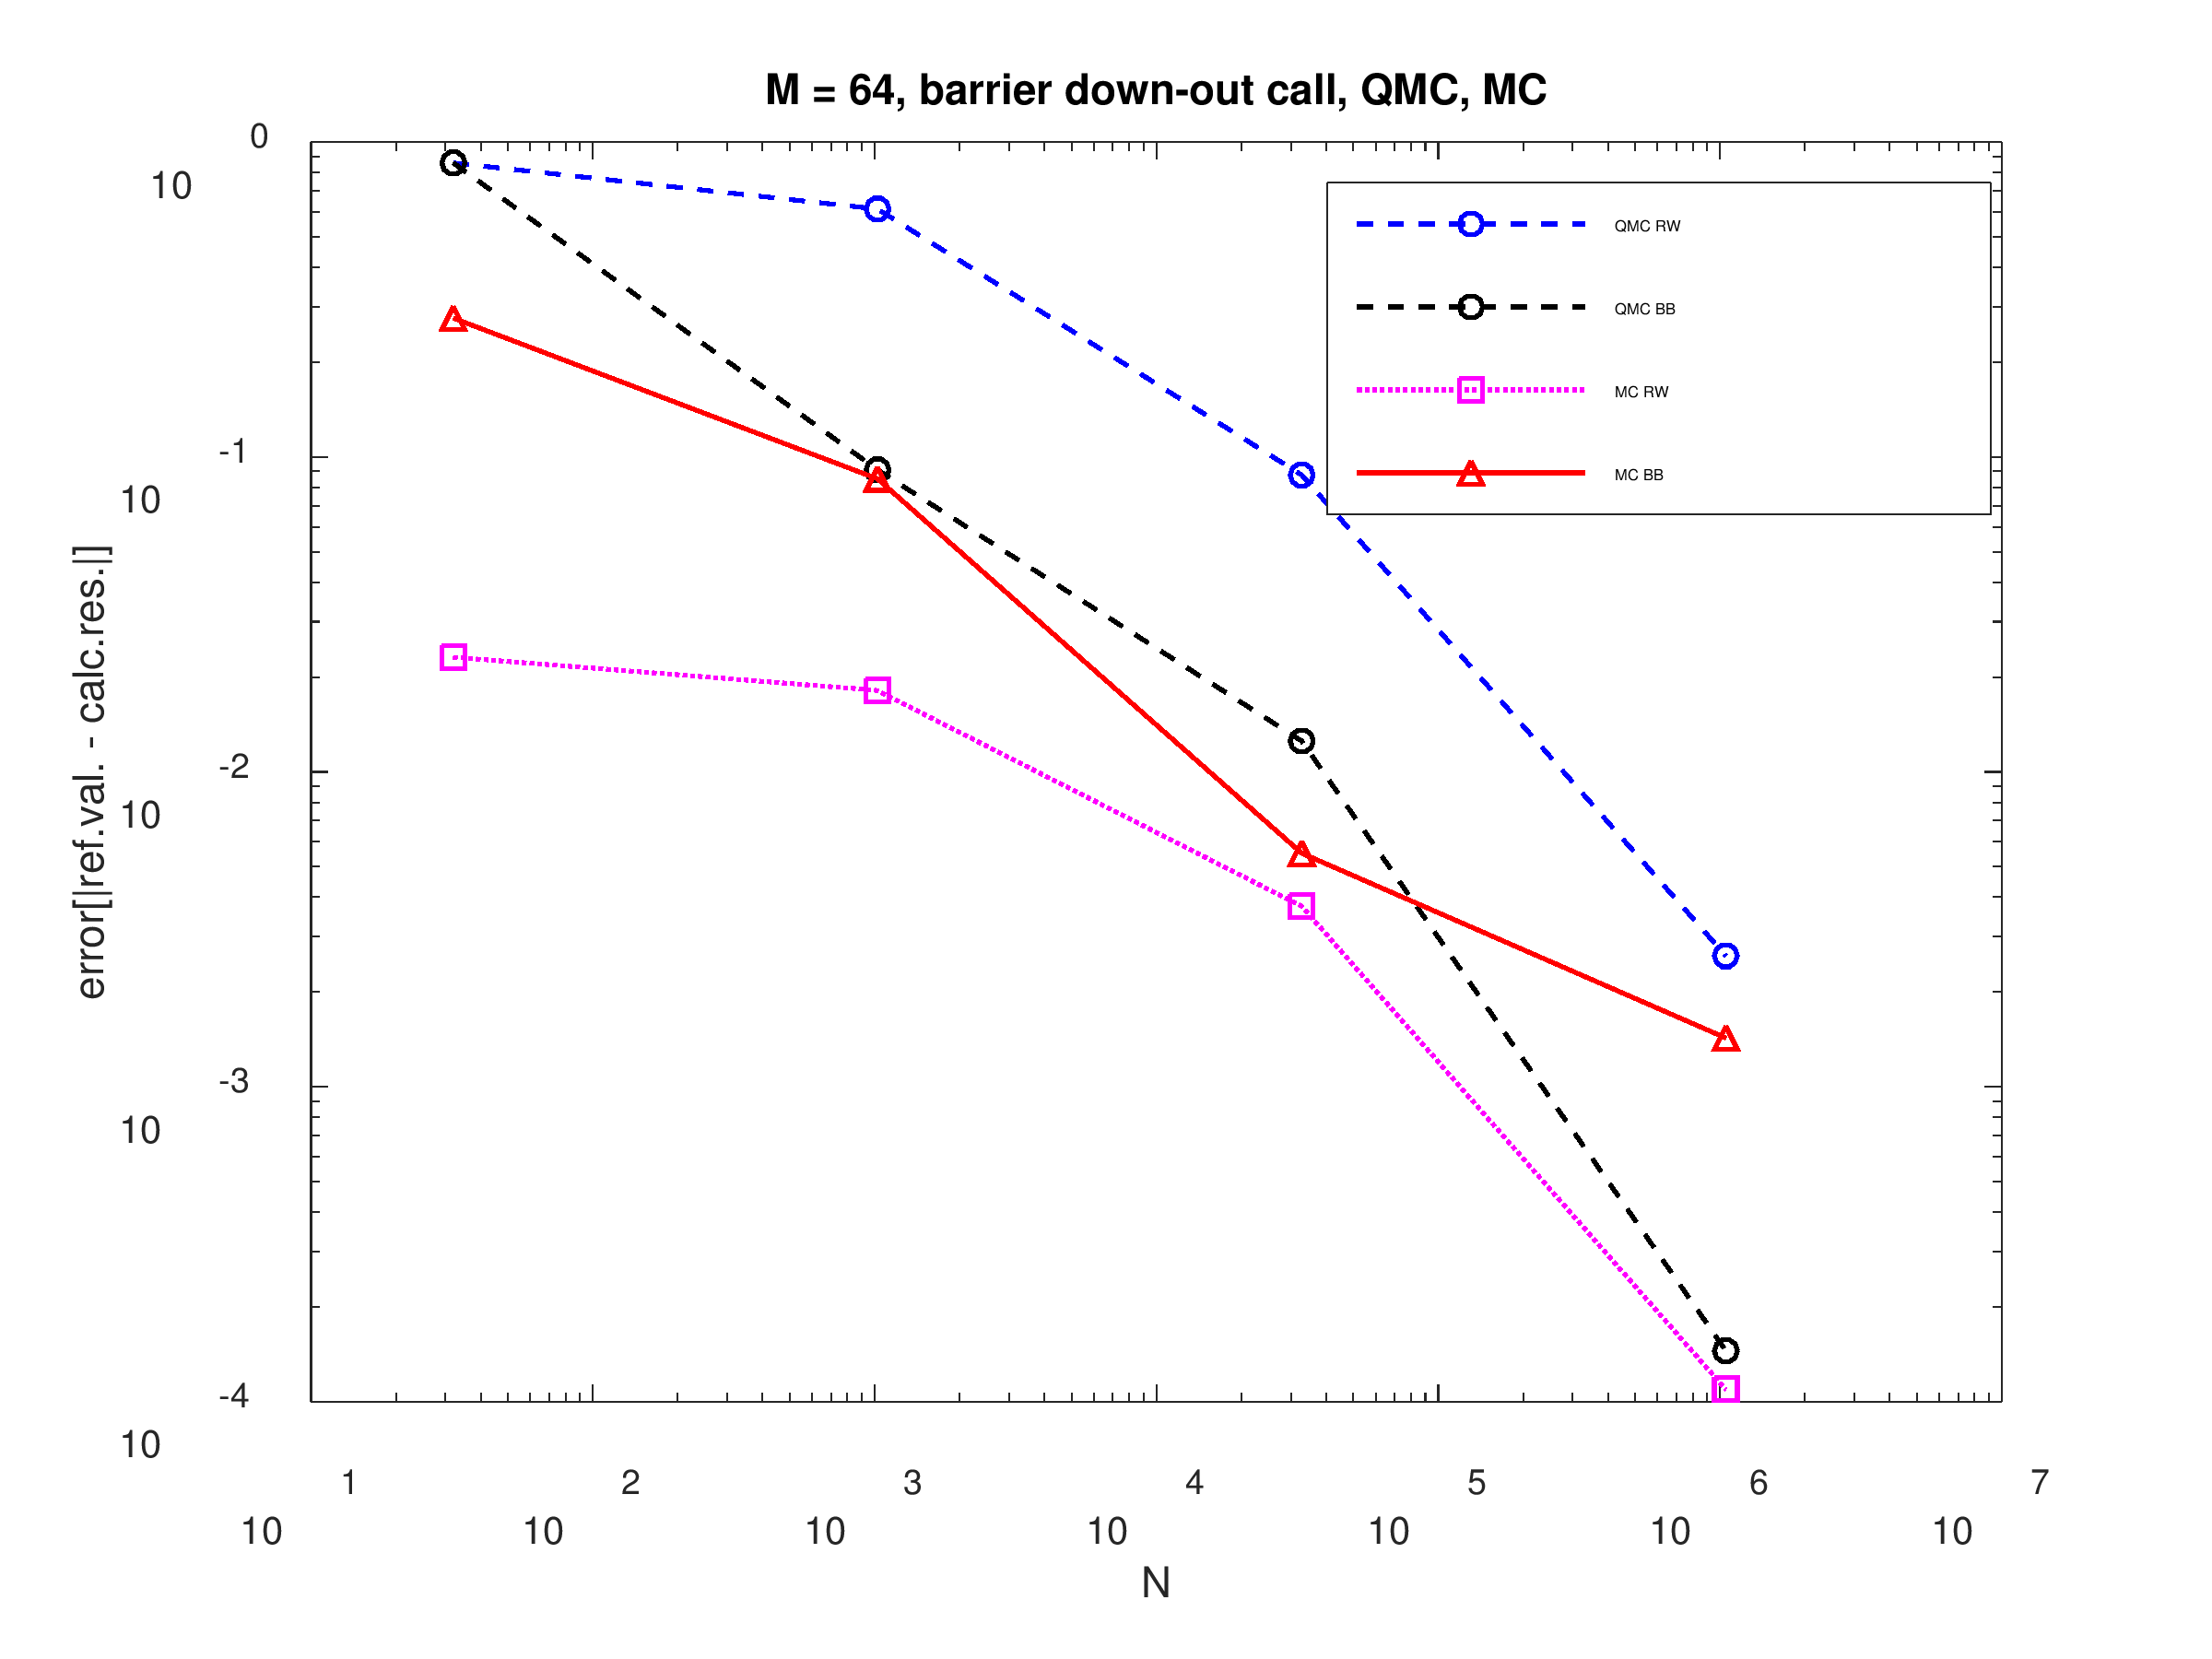
\includegraphics[scale=0.25]{images/task2_error.png}
\end{center}

\begin{itemize}
    \item{On this figure the absolute error: $|ref.val.-calc.val.|$ using different methods(QMC,MC) for Barrier Down-Out Call Option is plotted in loglog-scala against number of points.
    }
\item{
From the plots, one can observe that there is no really difference between using Brownian-Bridge or Random-Walk constructions.
}

\begin{center}
	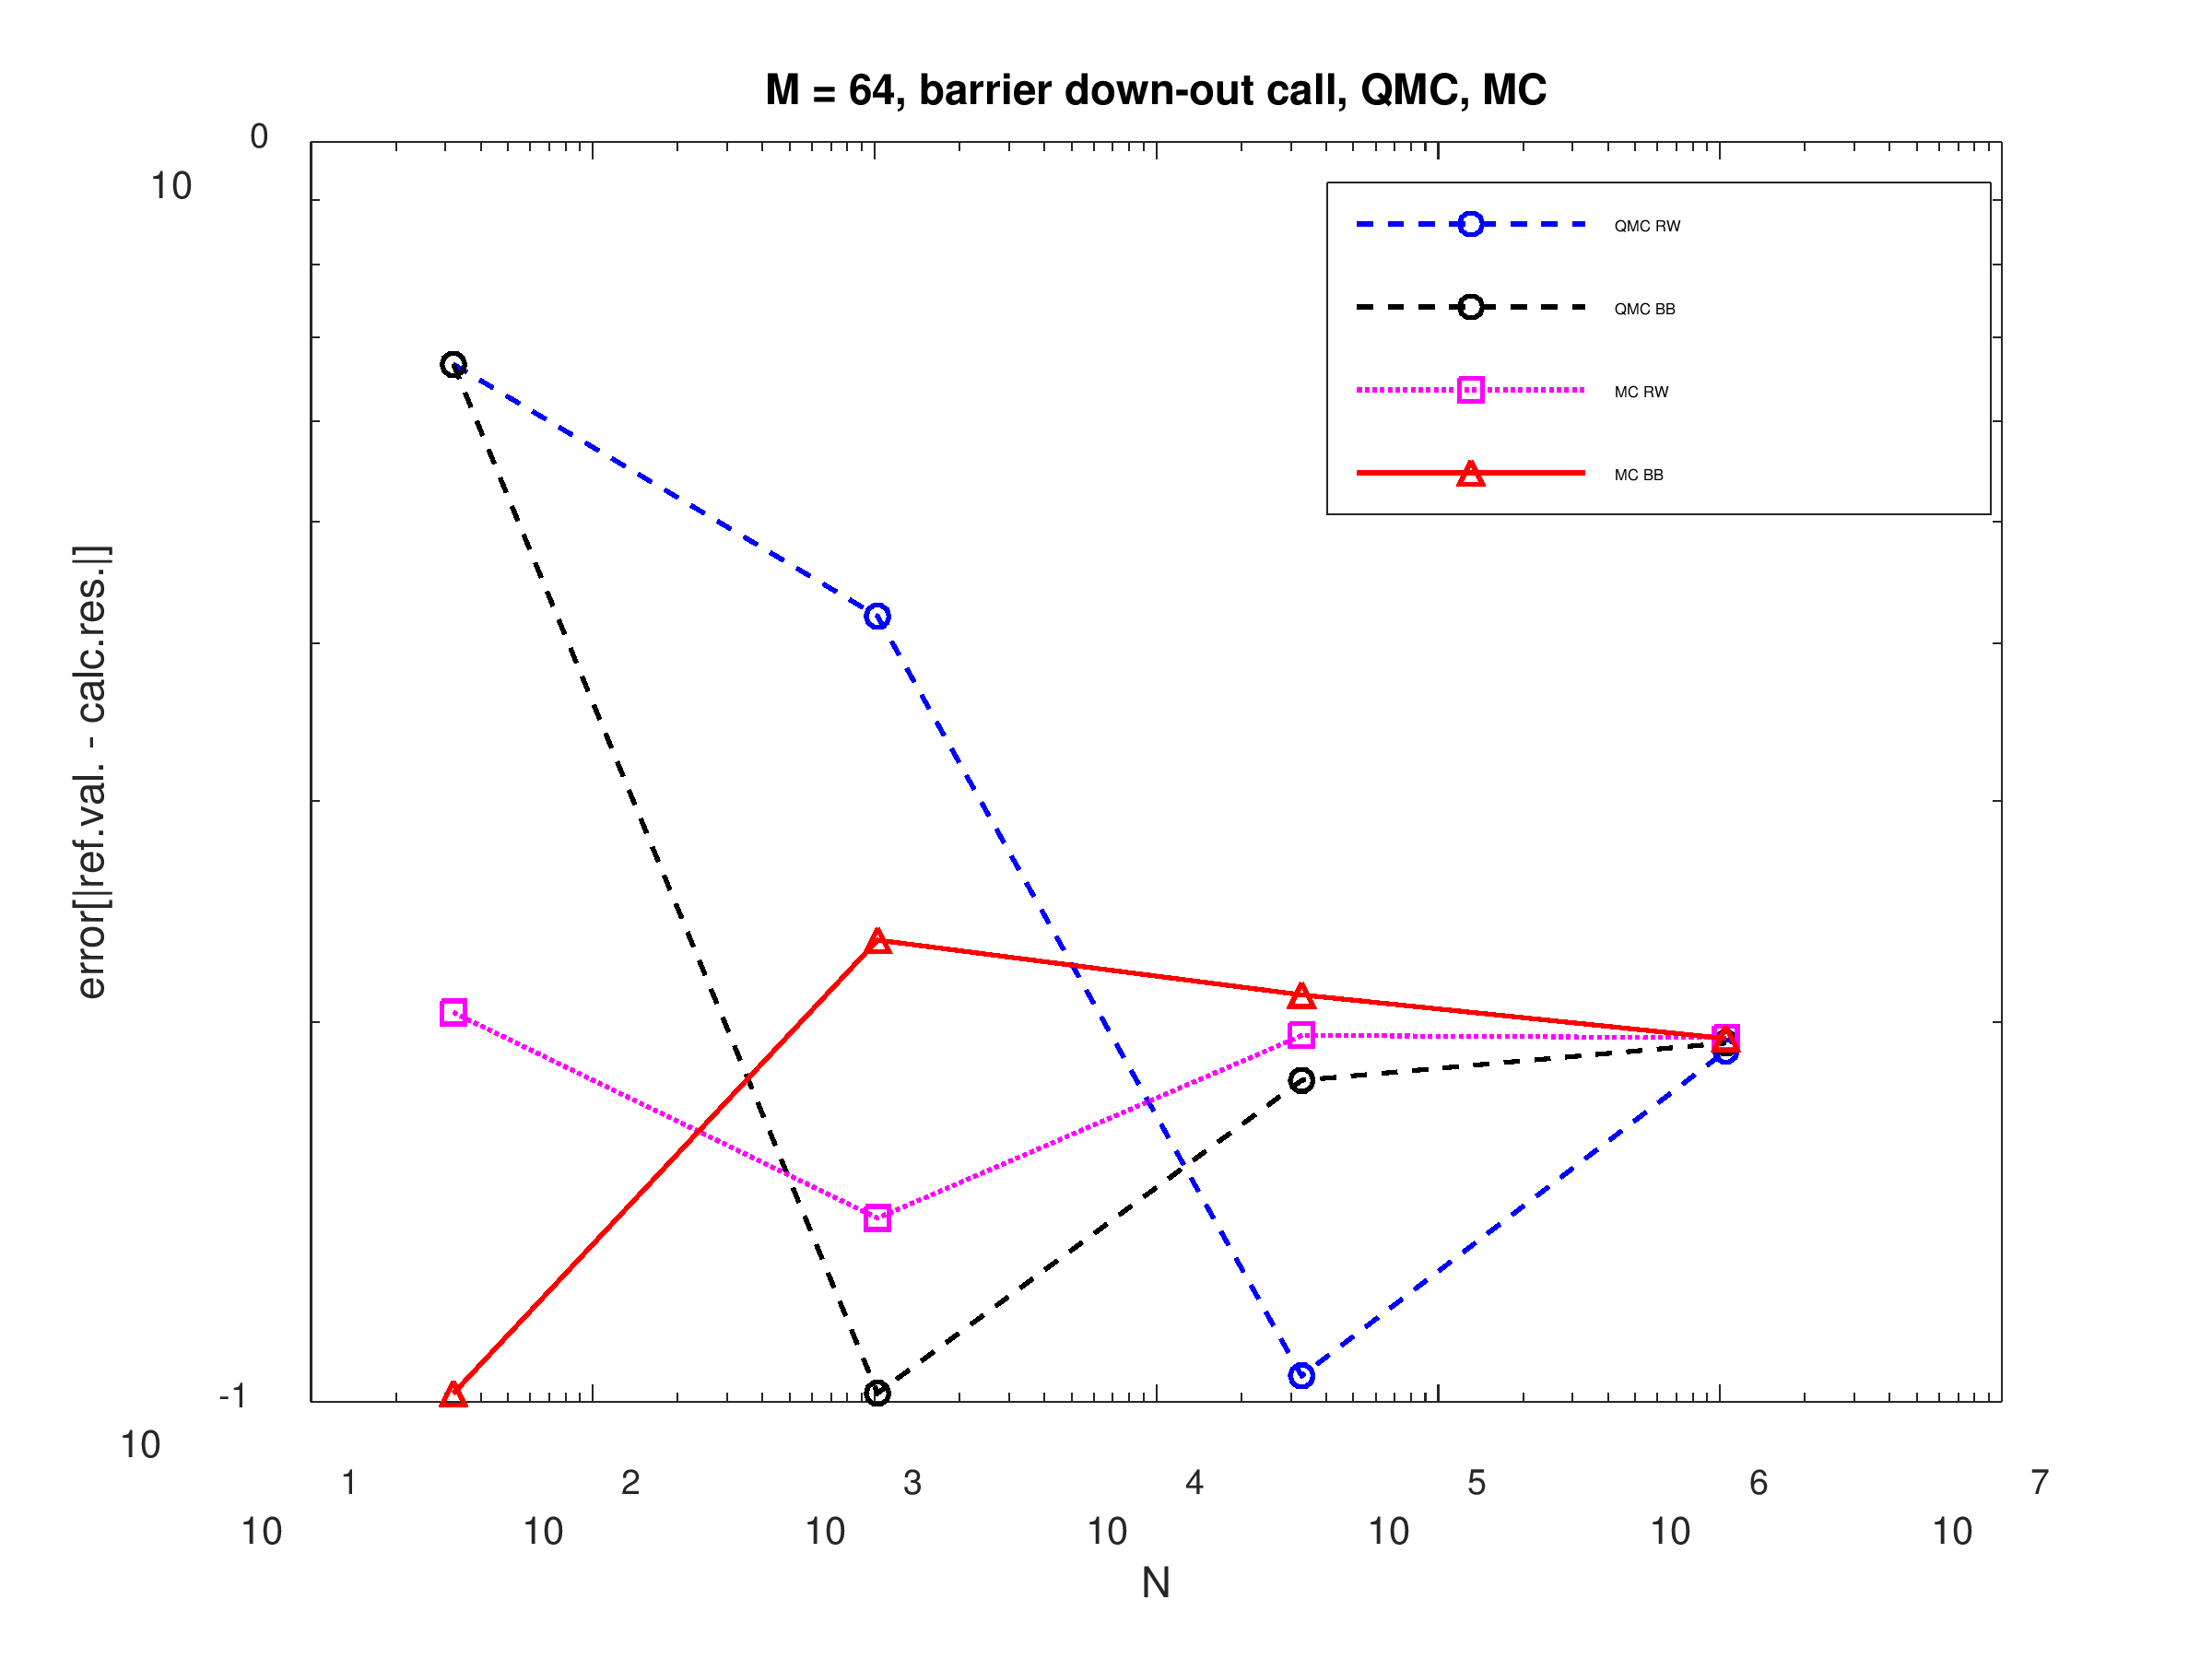
\includegraphics[scale=0.25]{images/task2_error_coarse_discretisation.png}
\end{center}
\item{
On this figure the absolute error: $|ref.val.-calc.val.|$ using different methods(QMC,MC) for Barrier Down-Out Call Option is plotted in loglog-scala against number of points. However now, reference value was computed using far more lower precision, where-from there is no convergence. 
}

\end{itemize}


\section*{Task 3}

The picture below shows the fair price for a Down-Out call option with barrier $B$. One can see that the fair price is going down if the barrier is larger then about $B=8$. This makes sense, because when the barrier is high, the payoff is $0$ in many cases (because for this value of $B$ it happens more often that the price of the underlying is below the barrier).

\begin{center}
	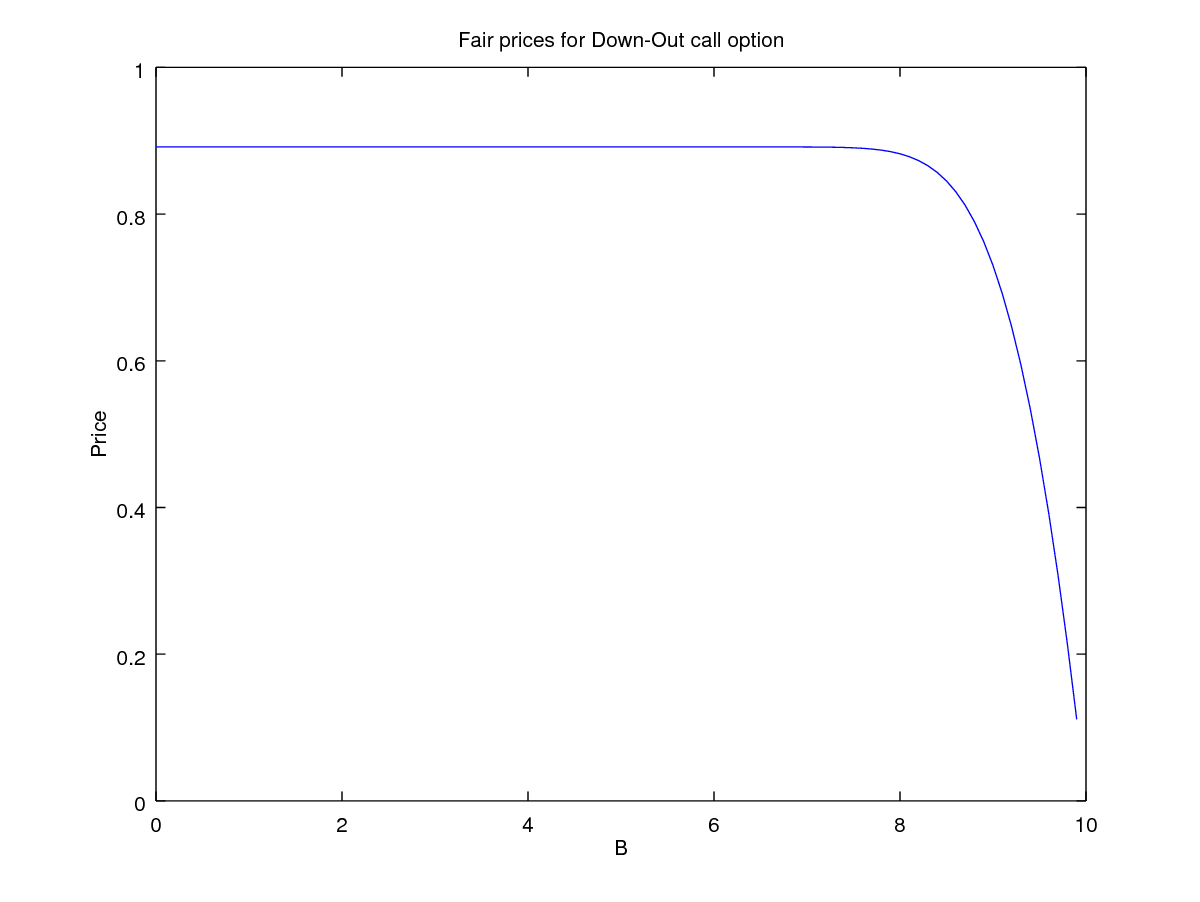
\includegraphics[scale=0.5]{images/fair_prices_down_out_call.png}
\end{center}

\section*{Task 4}
The next plot shows the absolute error for the discrete Down-Out call option for different values of $M$. One can see that for $M\geq64$ the convergence is much better then for $M=4$.  

\begin{center}
	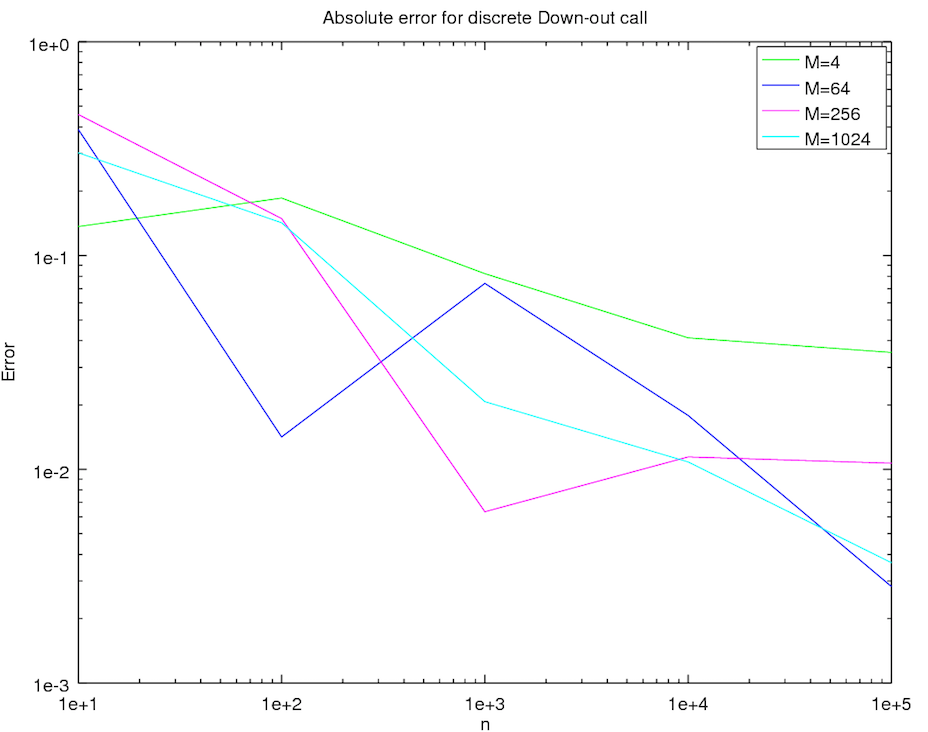
\includegraphics[scale=0.55]{images/convergence_plot_discrete_down_out_call.png}
\end{center}

\section*{Task 5}

\begin{center}
	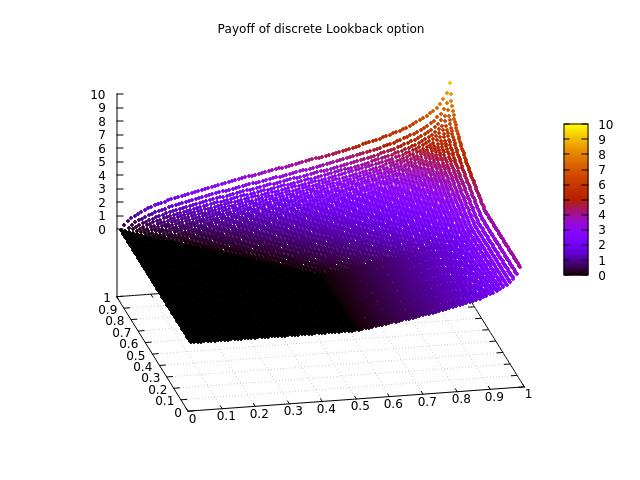
\includegraphics[scale=0.4]{images/payoff_lookback.png}
\end{center}

\section*{Task 6}

\begin{center}
	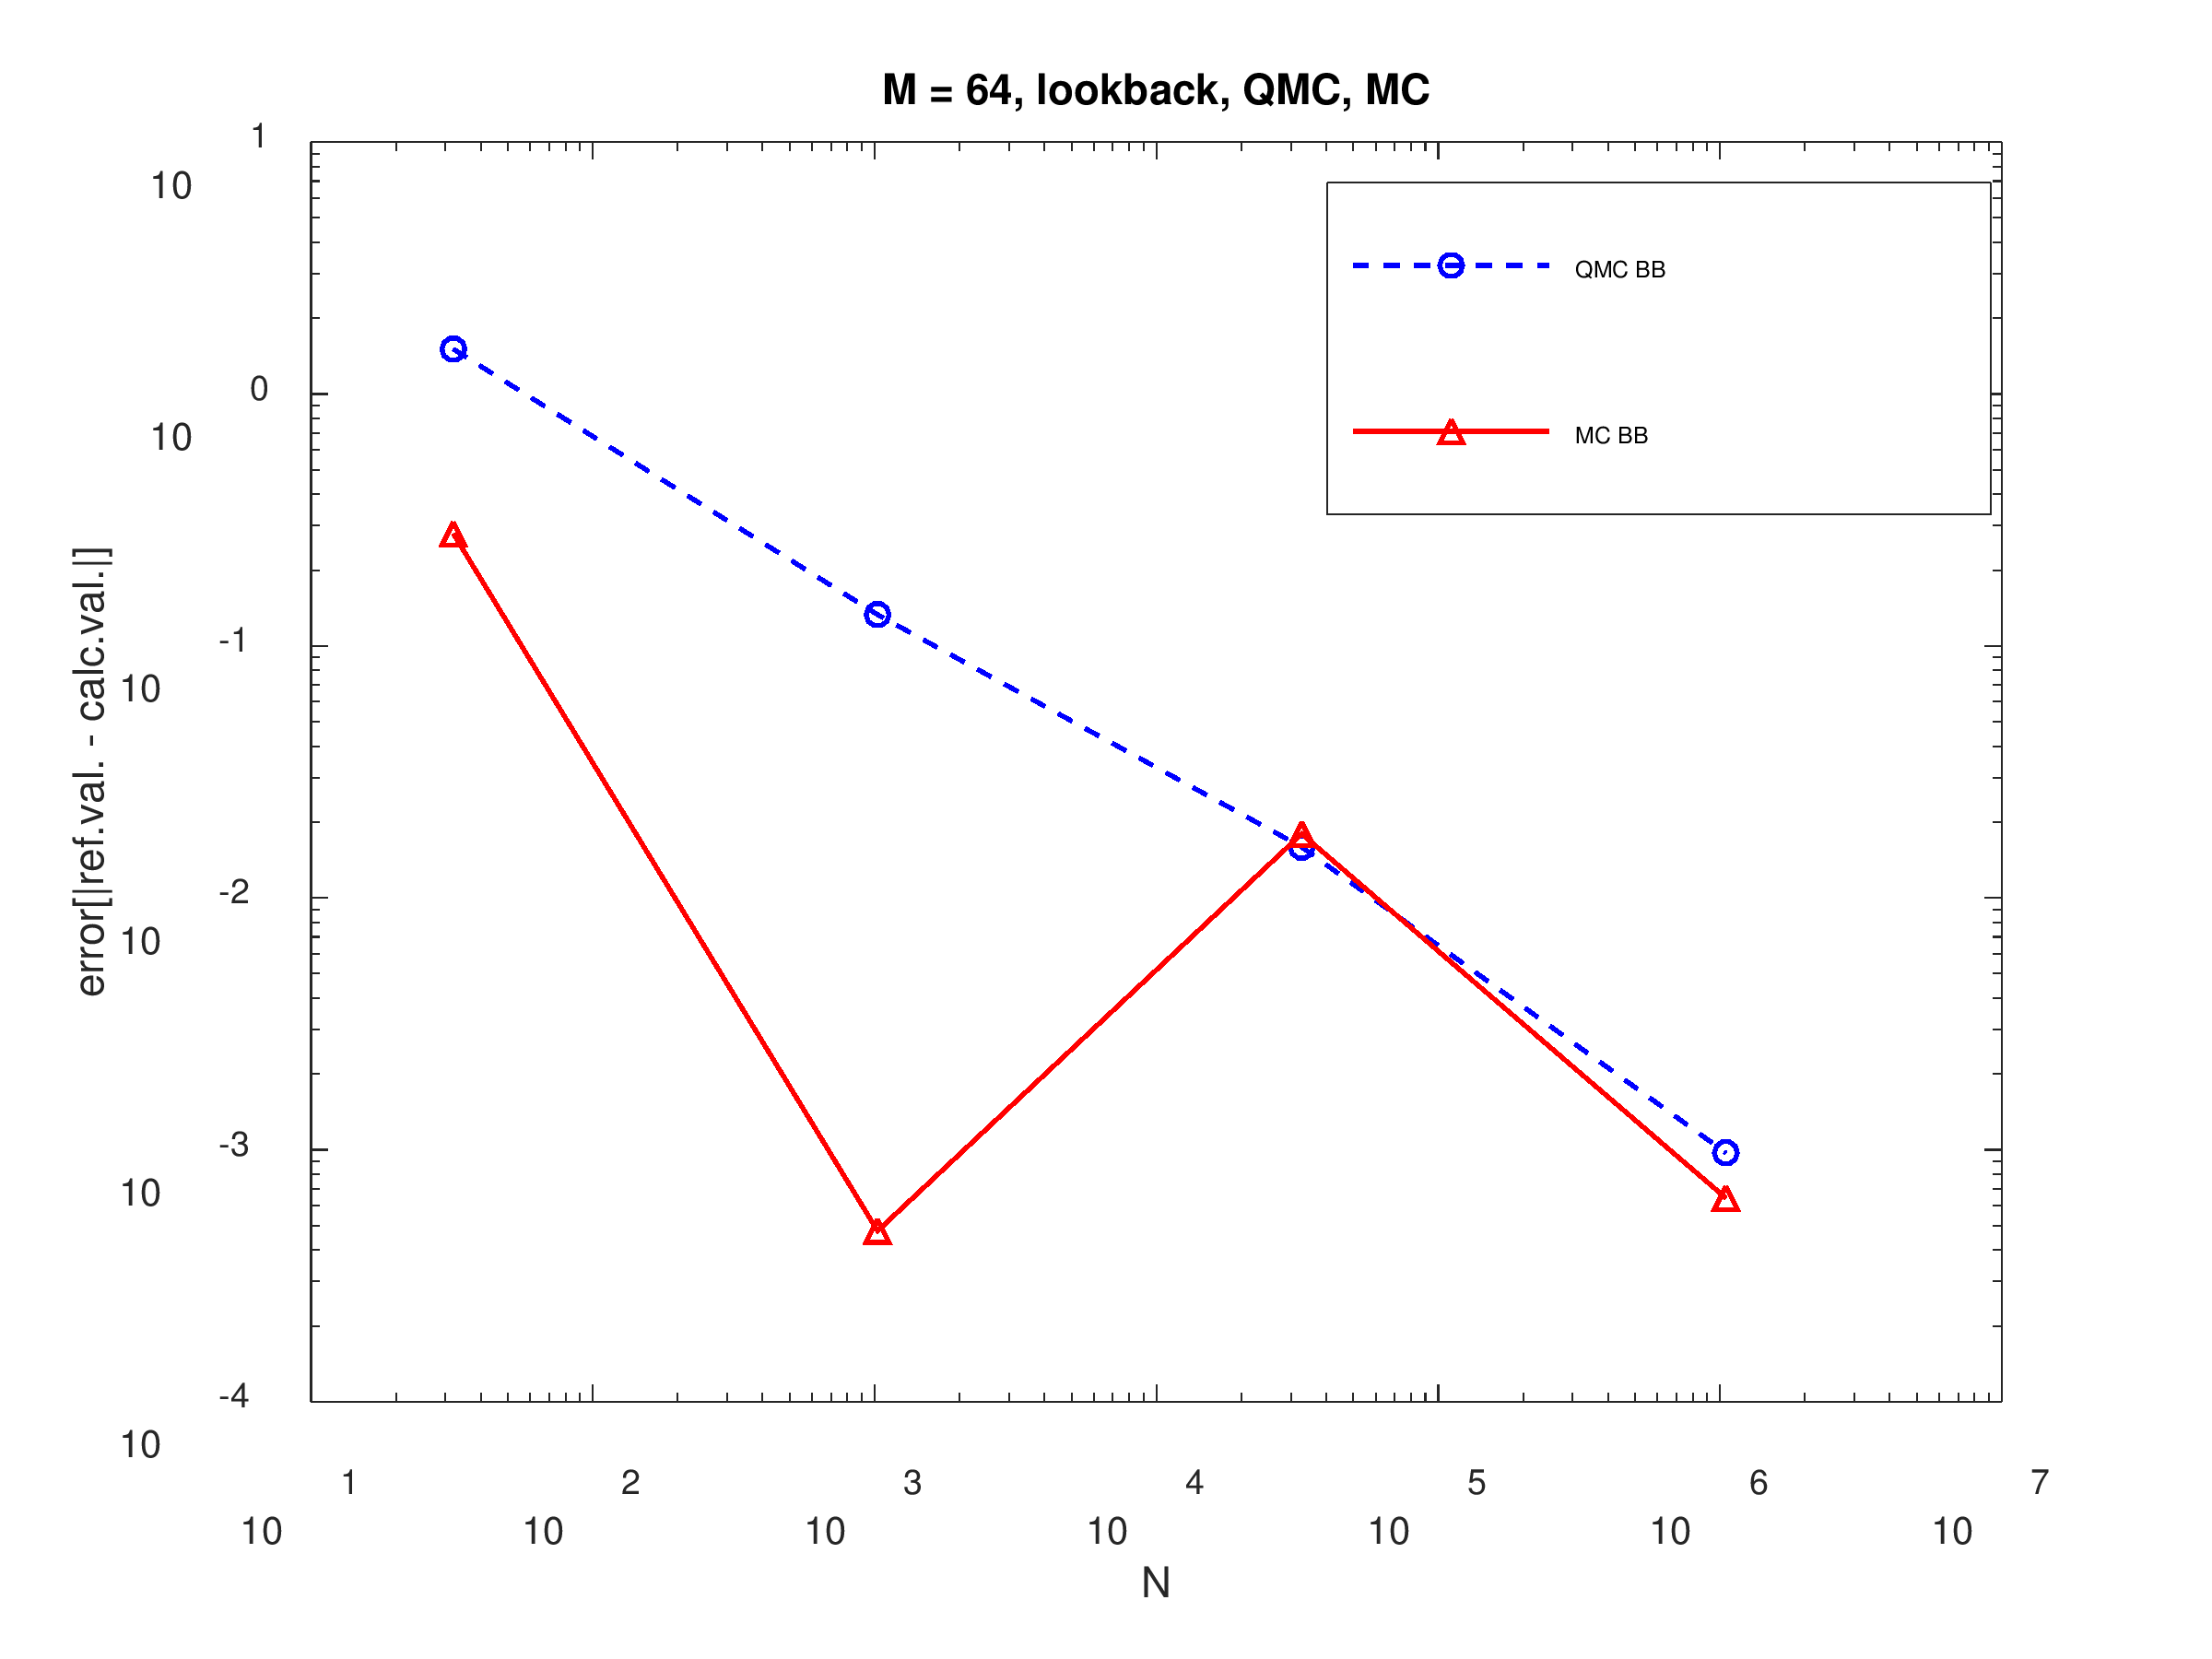
\includegraphics[scale=0.3]{images/task6_error.png}
\end{center}
\begin{itemize}
    \item{
        On this figure the absolute error: $|ref.val.-calc.val.|$ using different methods(QMC,MC with Brownian-Bridge) for Lookback Call Option is plotted in loglog-scala against number of points.
        
    }
     
\end{itemize}


\section*{Task 7}


\begin{center}
	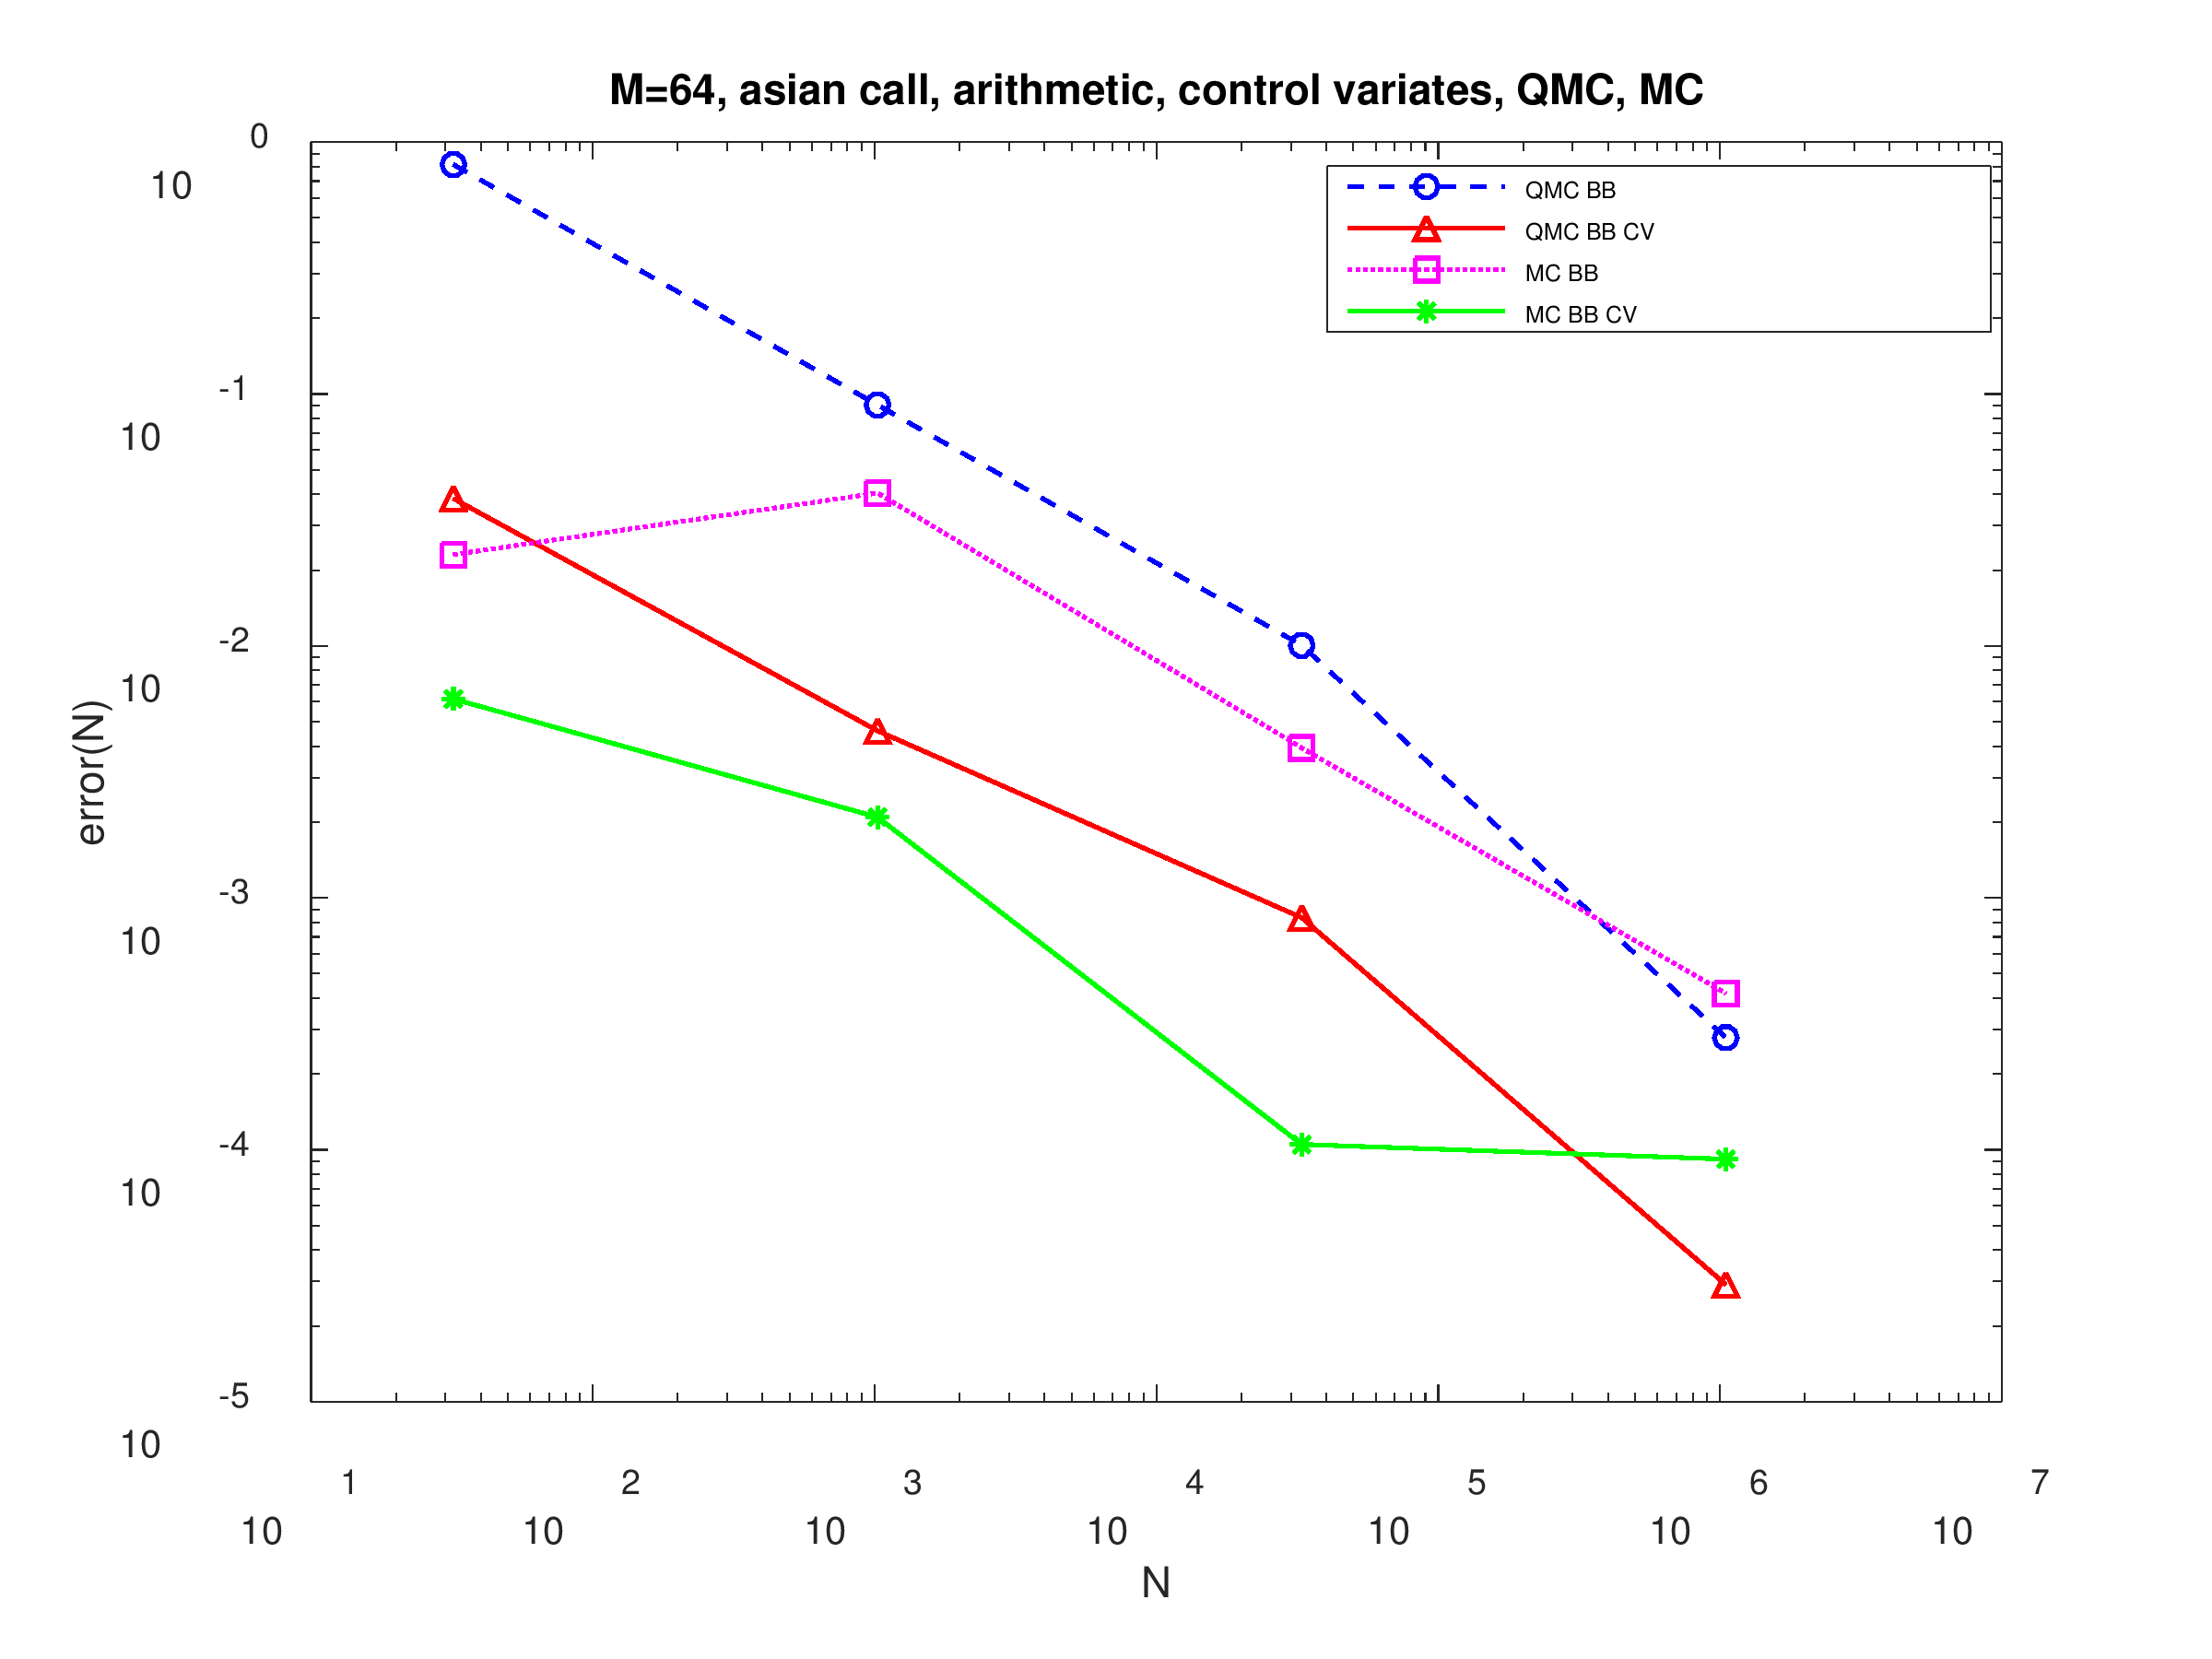
\includegraphics[scale=0.25]{images/task7_error.png}
\end{center}
\begin{itemize}
    \item{
        On this figure, results of the \textbf{control variate}
        method are presented. 
    }
\end{itemize}

\section*{Task 9}

\begin{center}
	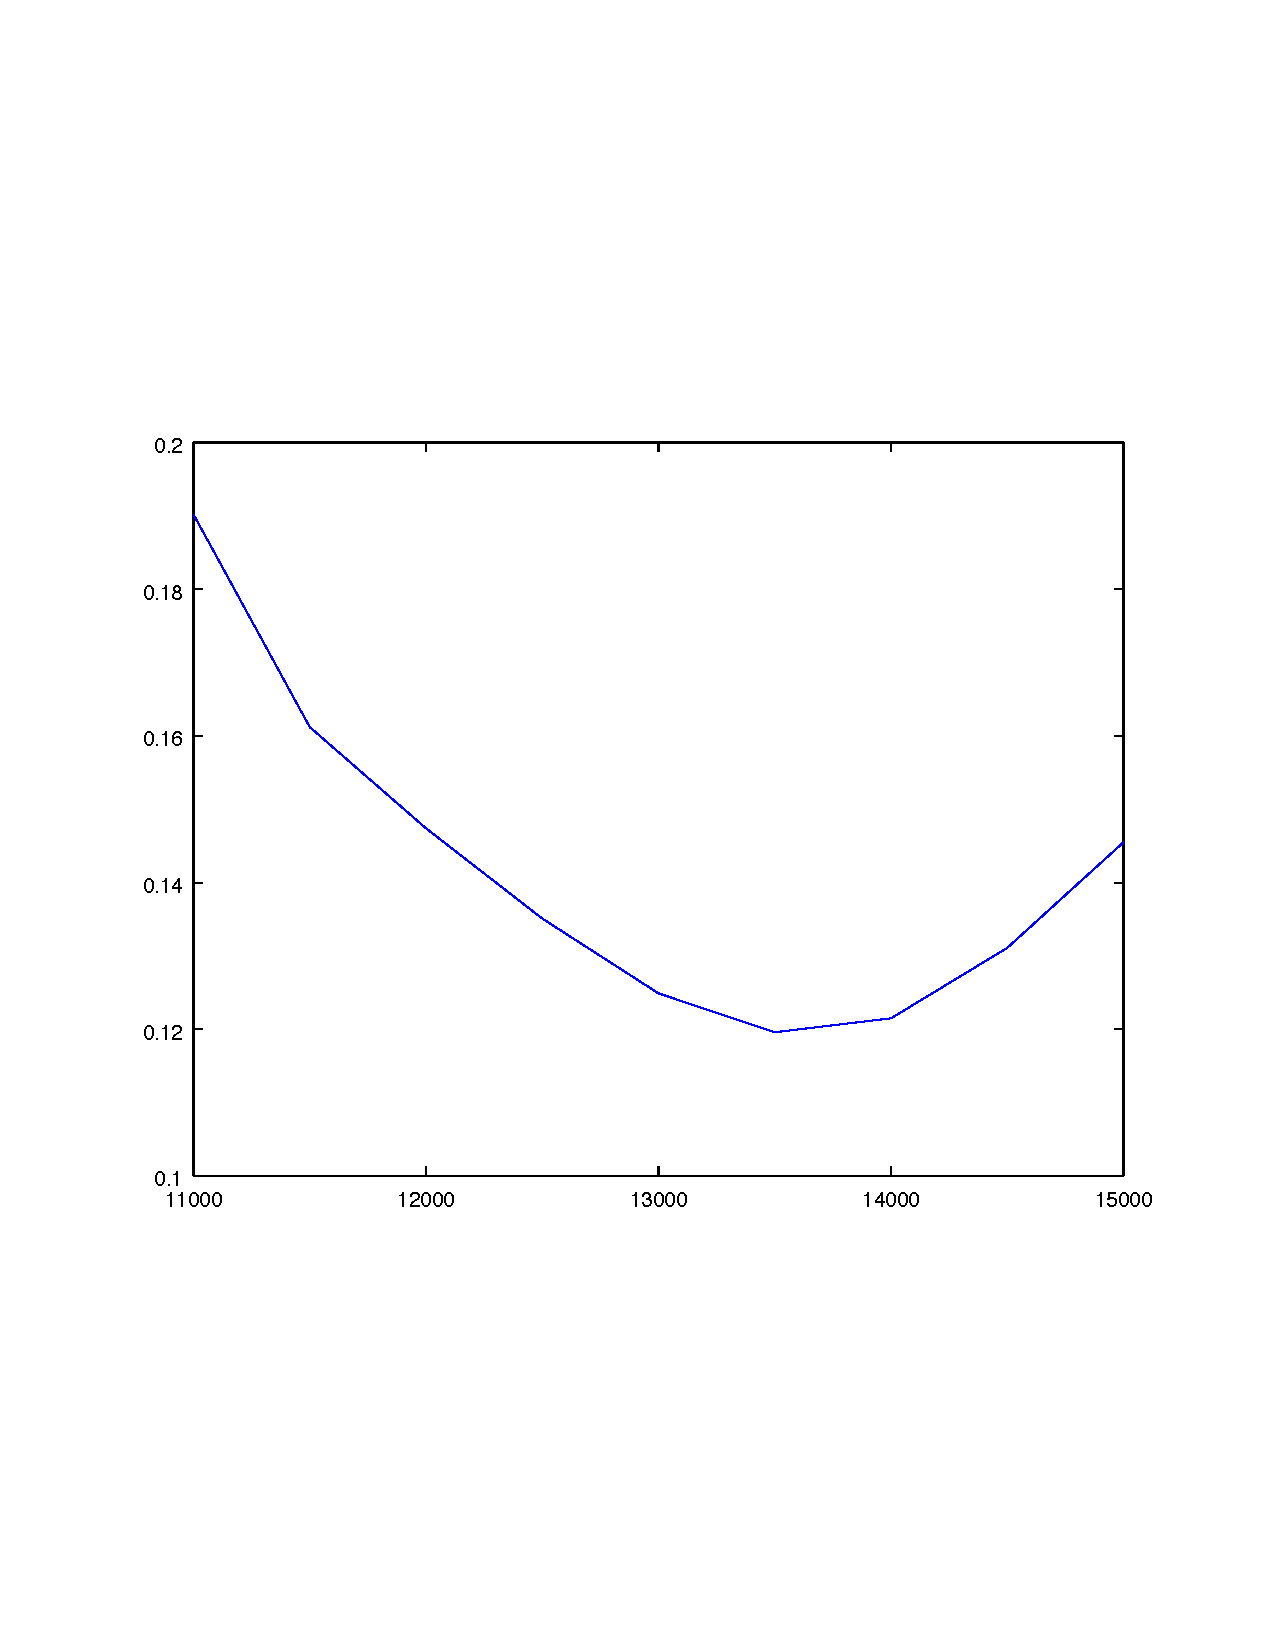
\includegraphics[scale=0.45]{images/dax.pdf}
\end{center}

Volatility of Call-Options for DAX, expiring in December, 2017. In this case, the volatility smile is clearly visible. The current value of the DAX is at about $12450$ points. 

\end{document}

